% begin module limit-def
\begin{frame}
\frametitle{The Limit of a Function}
\begin{definition}[The Limit of a Function]
We write
\[
\lim_{x\rightarrow a} f(x) = L
\]
and say ``the limit of $f(x)$, as $x$ approaches $a$, equals $L$,'' if we can make the values of $f(x)$ arbitrarily close to $L$ by taking $x$ to be sufficiently close to $a$ (on either side of $a$) but not equal to $a$.
\end{definition}
\begin{center}
\ \only<handout:0| -1>{%
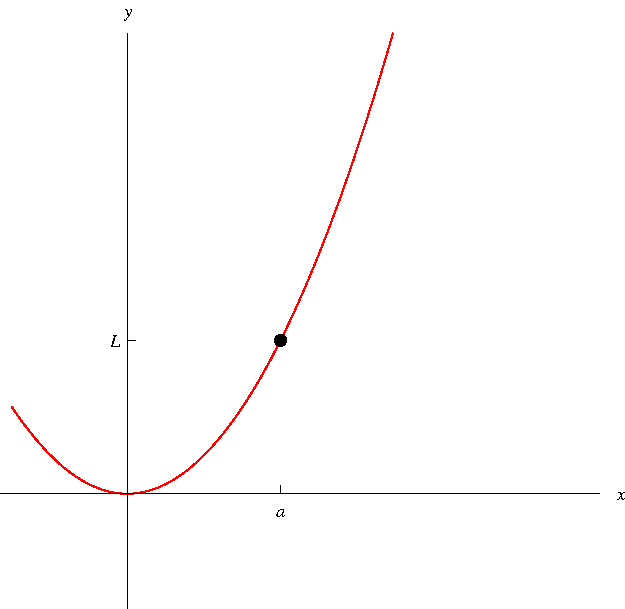
\includegraphics[height=4cm]{limits/pictures/02-01-limita.pdf}%
}%
\only<handout:0| 2>{%
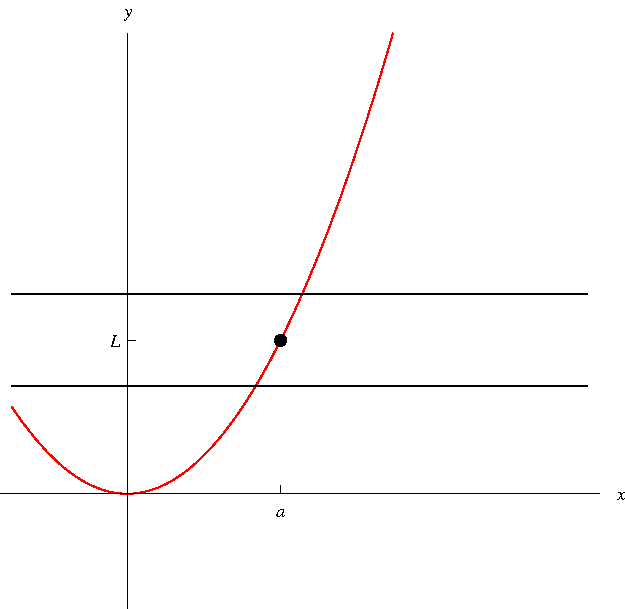
\includegraphics[height=4cm]{limits/pictures/02-01-limitb.pdf}%
}%
\only<3->{%
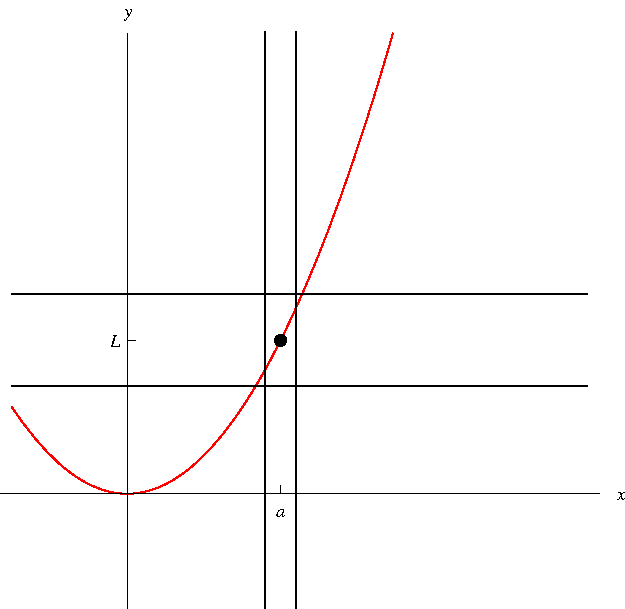
\includegraphics[height=4cm]{limits/pictures/02-01-limitc.pdf}%
}%
\end{center}
\end{frame}
% end module limit-def
